
We wish to solve the advection-diffusion problem presented in 
Section~\ref{ss:advdiff}:
\begin{equation}
\rho C_p u \frac{dT}{dx} - k \frac{d^2T}{dx^2} = f \qquad \text{in} \quad [0,L_x]
\end{equation}
with the boundary conditions $T(x=0)=0$ and $T(x=L_x)=0$.

The domain is characterised by $L_x=1$, and since $L_y$ is irrelevant it is set to $L_x/10$.
We further set $nelx=10$, $f=1$, $\rho=1$, $C_p=1$, $u=1$.
We will consider three values of the Peclet number: 0.25, 1 and 5.
From these values we can compute the corresponding heat conductivity value $k$.
Linear elements are used.

As $Pe$ increases, a sharp gradient, sometimes called a boundary layer,
develops at the right end of the domain. For high $Pe$ values, the solution shows 
spurious node to node oscillations, failing to capture the highly nonlinear change. This oscillatory
behavior is seen for $Pe>1$ (see Donea \& Huerta \cite{dohu03}).

\begin{center}
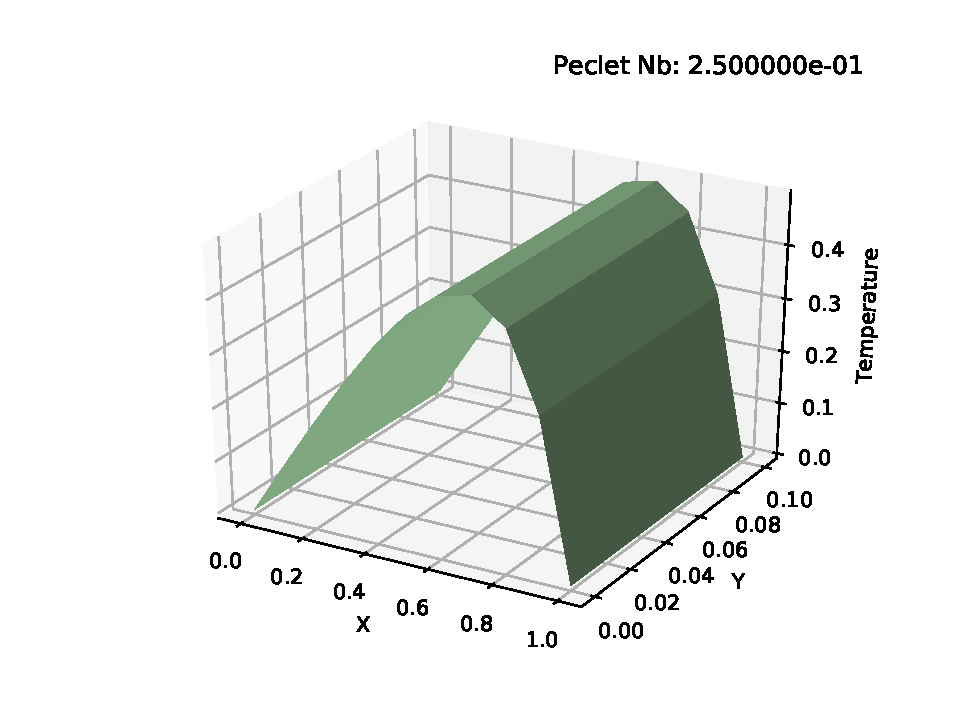
\includegraphics[width=5cm]{python_codes/fieldstone_65/results/solution1.pdf}
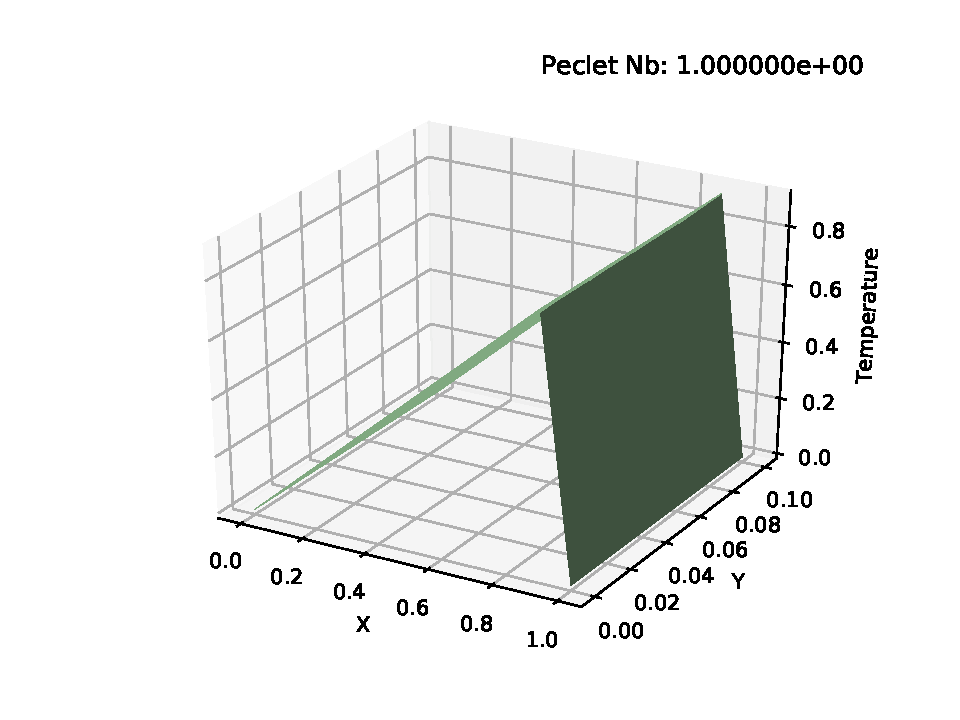
\includegraphics[width=5cm]{python_codes/fieldstone_65/results/solution2.pdf}
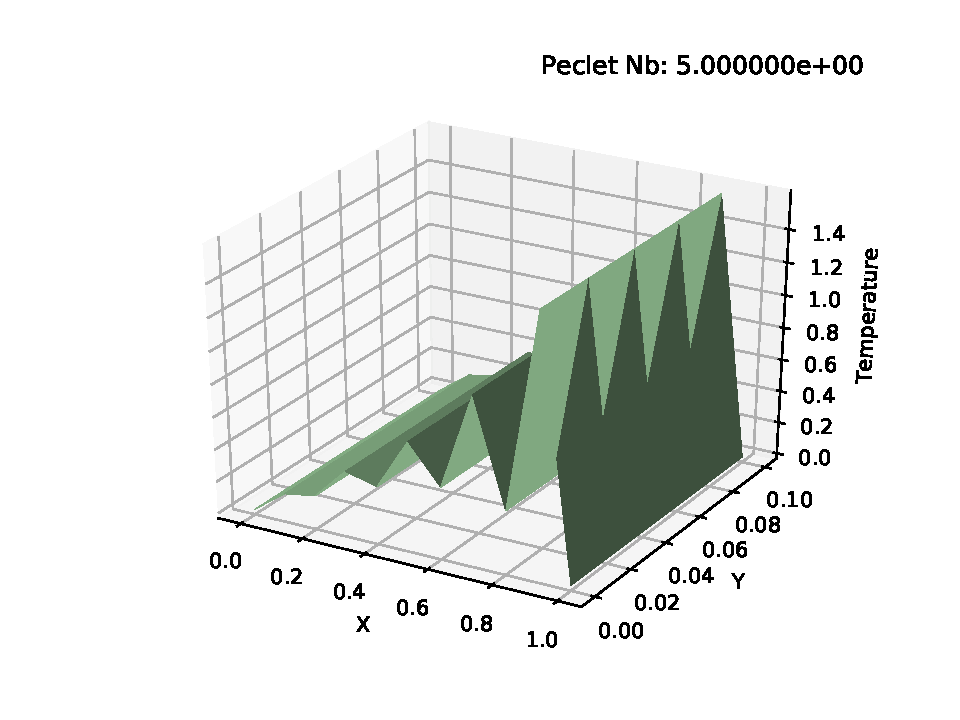
\includegraphics[width=5cm]{python_codes/fieldstone_65/results/solution3.pdf}\\
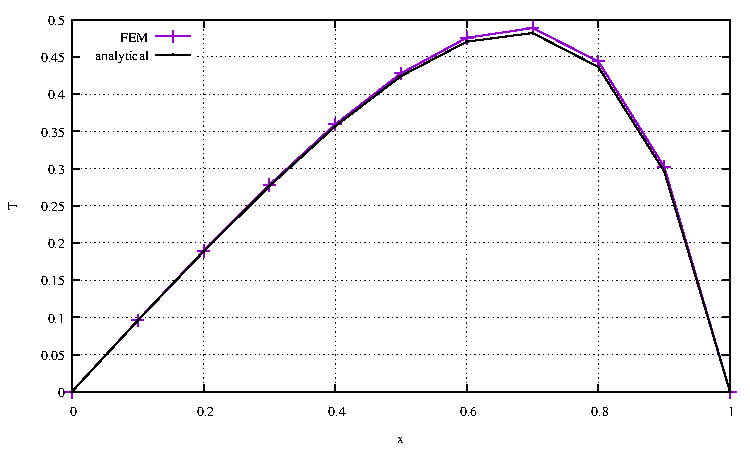
\includegraphics[width=5cm]{python_codes/fieldstone_65/results/T1.pdf}
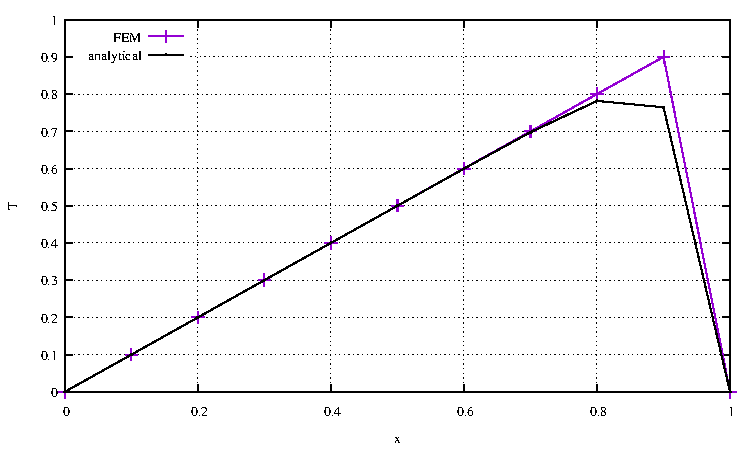
\includegraphics[width=5cm]{python_codes/fieldstone_65/results/T2.pdf}
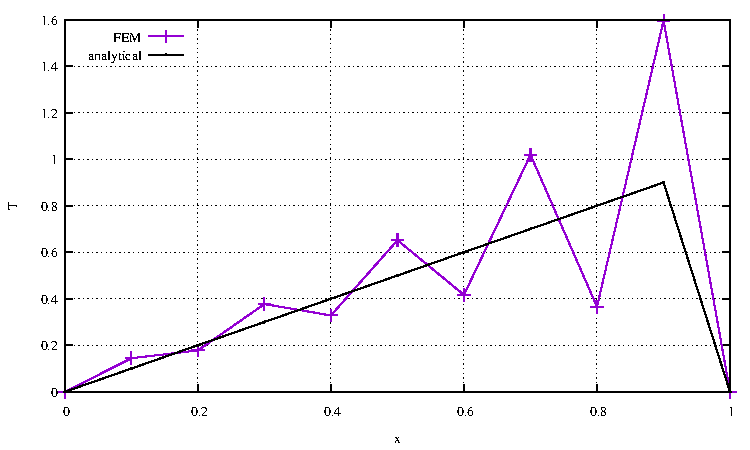
\includegraphics[width=5cm]{python_codes/fieldstone_65/results/T3.pdf}\\
{\captionfont Left to right: $Pe$=0.25, $Pe$=1, $Pe$=5}
\end{center}

Finally we see that we recover identical results as in Donea \& Huerta \cite{dohu03}:

\begin{center}
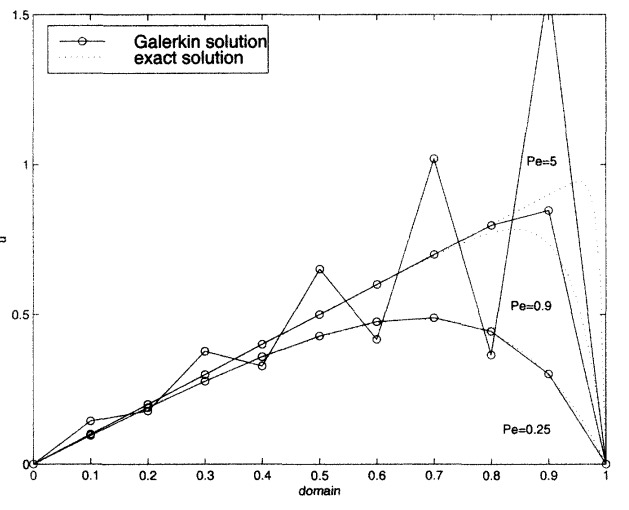
\includegraphics[width=8cm]{python_codes/fieldstone_65/images/dohu}
\end{center}

